\documentclass{elsarticle}
\usepackage[T1]{fontenc}
\usepackage{amsmath}
\usepackage{amssymb}
\usepackage{xcolor,colortbl}
\usepackage{tikz}
\usetikzlibrary{calc}
\usetikzlibrary{shapes.geometric}

\begin{document}

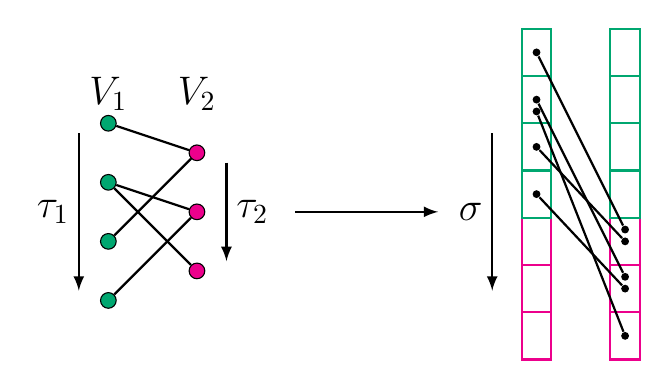
\begin{tikzpicture}
\begin{scope}[scale=0.75]
\node [circle, fill=cyan!20!green, draw=black,  inner sep=2pt] (v1) at (-4.5,4) {};
\node [circle, fill=cyan!20!green, draw=black,  inner sep=2pt] (v4) at (-4.5,3) {};
\node [circle, fill=cyan!20!green,draw=black,    inner sep=2pt] (v7) at (-4.5,1) {};
\node [circle, fill=cyan!20!green, draw=black,   inner sep=2pt] (v3) at (-4.5,2) {};
\node [circle, fill=magenta, draw=black,  inner sep=2pt] (v2) at (-3,3.5) {};
\node [circle, fill=magenta, draw=black,  inner sep=2pt] (v5) at (-3,2.5) {};
\node [circle, fill=magenta, draw=black,  inner sep=2pt] (v6) at (-3,1.5) {};
\draw [thick, color=black] (v1) edge (v2);
\draw [thick, color=black] (v2) edge (v3);
\draw [thick, color=black] (v4) edge (v5);
\draw [thick, color=black] (v4) edge (v6);
\draw [thick, color=black] (v5) edge (v7);
\node[draw=none, text=black] at (-4.5,4.5){\Large $V_1$};
\node[draw=none, text=black] at (-3,4.5){\Large $V_2$};
\node (v1) at (-5,4) {};
\node (v2) at (-5,1) {};
\draw[thick, color=black, -{latex[scale=1.5]}](v1)--(v2);
\node[draw=none, text=black, left] at (-5,2.5){\Large $\tau_1$};
\node (v3) at (-2.5, 3.5){};
\node (v4) at (-2.5, 1.5){};
\draw[thick, color=black, -{latex[scale=1.5]}](v3)--(v4);
\node[draw=none, text=black, right] at (-2.5,2.5){\Large $\tau_2$};
\node (v8) at (-1.5,2.5) {};
\node (v9) at (1.25,2.5) {};
\draw [thick, color=black, -{latex[scale=1.5]}] (v8) edge (v9);
\node (v10) at (2,4) {};
\node  (v11) at (2,1) {};
\draw [thick, color=black, -{latex[scale=1.5]}] (v10) edge (v11);
\node[draw=none, text=black, left] at (2,2.5){\Large $\sigma$};
\draw [thick, magenta] (2.5,0) rectangle (3,2.4);
\draw [thick, magenta] (2.5,0.8)--(3,0.8);
\draw [thick, magenta] (2.5, 1.6)--(3, 1.6);
\draw [thick, cyan!20!green] (2.5,2.4) rectangle (3,5.6);
\draw [thick, cyan!20!green] (2.5,3.2)--(3,3.2);
\draw [thick, cyan!20!green] (2.5, 4)--(3, 4);
\draw [thick, cyan!20!green] (2.5, 4.8)--(3, 4.8);

\draw [thick, magenta] (4,0) rectangle (4.5,2.4);
\draw [thick, magenta] (4,0.8)--(4.5,0.8);
\draw [thick, magenta] (4, 1.6)--(4.5, 1.6);
\draw [thick, cyan!20!green] (4,2.4) rectangle (4.5,5.6);
\draw [thick, cyan!20!green] (4,3.2)--(4.5,3.2);
\draw [thick, cyan!20!green] (4, 4)--(4.5, 4);
\draw [thick, cyan!20!green] (4, 4.8)--(4.5, 4.8);
\node [circle, fill=black,  inner sep=1pt] (v12) at (2.75,5.2) {};
\node [circle, fill=black,  inner sep=1pt] (v14) at (2.75,4.4) {};
\node [circle, fill=black,  inner sep=1pt] (v16) at (2.75,4.2) {};
\node [circle, fill=black,  inner sep=1pt] (v18) at (2.75,3.6) {};
\node [circle, fill=black,  inner sep=1pt] (v20) at (2.75,2.8) {};
\node [circle, fill=black,  inner sep=1pt] (v13) at (4.25,2.2) {};
\node [circle, fill=black,  inner sep=1pt] (v19) at (4.25,2) {};
\node [circle, fill=black,  inner sep=1pt] (v15) at (4.25,1.4) {};
\node [circle, fill=black,  inner sep=1pt] (v21) at (4.25,1.2) {};
\node [circle, fill=black,  inner sep=1pt] (v17) at (4.25,0.4) {};
\draw [thick, color=black] (v12) edge (v13);
\draw [thick, color=black] (v14) edge (v15);
\draw [thick, color=black] (v16) edge (v17);
\draw [thick, color=black] (v18) edge (v19);
\draw [thick, color=black] (v20) edge (v21);
\end{scope}
\end{tikzpicture}

\end{document}